\documentclass[11pt,a4paper]{article}

\usepackage[margin=2.5cm]{geometry}
\usepackage[T1]{fontenc}
\usepackage{lmodern}
\usepackage{microtype}
\usepackage{amsmath,amssymb,amsthm,bm}
\usepackage{booktabs}
\usepackage{enumitem}
\usepackage{tikz}
\usetikzlibrary{arrows.meta,positioning}
\usepackage[colorlinks=true,linkcolor=blue!50!black,citecolor=blue!50!black,urlcolor=blue!50!black]{hyperref}

\newcommand{\vect}[1]{\bm{#1}}
\newcommand{\x}{\vect{x}}
\newcommand{\X}{\vect{X}}
\newcommand{\uu}{\vect{u}}
\newcommand{\R}{\vect{R}}
\newcommand{\K}{\mathbf{K}}
\newcommand{\g}{\vect{g}}
\newcommand{\n}{\vect{n}}
\newcommand{\I}{\mathbf{I}}
\newcommand{\dV}{\Delta V}
\newcommand{\code}[1]{\texttt{#1}}
\DeclareMathOperator{\tr}{tr}
\DeclareMathOperator{\diag}{diag}

\theoremstyle{remark}
\newtheorem*{remark}{Remark}

\title{\textbf{Membrane Neuron Simulator}\\[4pt]
\large Formulation and implementation of a static solver for fluid-driven membrane neurons}
\author{W.\,J.\ van Vuuren}
\date{Technical reference accompanying the source code\\
\url{https://github.com/vanvuurenwerner2305-blip/MechanicalNeuronSimulation}}

\begin{document}
\maketitle

\begin{abstract}
This document describes the mathematics and algorithms of the Membrane Neuron Simulator, the
software used to simulate the mechanical neurons of the accompanying thesis. A mechanical neuron
consists of thin rubber membranes that separate fluid chambers and deform against rigid parts.
The software imports such a device from CAD, models the membranes as geometrically nonlinear
shells, the chambers as volume-dependent pressure laws and the rigid parts as contact obstacles,
and solves for static equilibrium by minimising a total potential energy with a safeguarded
Newton method. From a sweep over the input pressures it then back-infers the neuron equation, in
the form of the mechanical weights of the neuron model, as low-degree piecewise polynomials.

None of the ingredients is new: the membrane and bending elements, the pressure loads, the
penalty contact and the Newton globalisation are standard techniques from the literature, cited
where they are used. The purpose of this document is to state exactly which formulation the code
implements, so that the results in the thesis can be reproduced and checked.
\end{abstract}

\tableofcontents
\newpage

%=====================================================================
\section{Scope and overview}
%=====================================================================

The simulator answers one question: \emph{given a device and the pressures in its input
chambers, what is the static equilibrium shape of its membranes, and what are the resulting
pressures in its sealed chambers?} The device is built in CAD (Fusion~360 in practice),
exported as a STEP file, and every solid body is given one of the following roles:
\begin{itemize}[noitemsep]
  \item \textbf{Membrane}: a thin solid with membrane stiffness only;
  \item \textbf{Shell}: a thin solid with membrane and bending stiffness;
  \item \textbf{Rigid body}: an obstacle that the membranes cannot penetrate;
  \item \textbf{Fluid chamber}: a solid that fills a fluid space, with a pressure model
        (constant-pressure input, sealed ideal gas, sealed liquid, or vent to the surroundings);
  \item \textbf{Ignore}.
\end{itemize}
Chamber walls are never meshed. Rigid bodies are meshed as closed surfaces, and membranes and
shells are replaced by triangulated mid-surfaces.

The whole analysis is \emph{quasi-static}. Nothing depends on time: there is no inertia, no
viscosity and no fluid flow. Every chamber is a lumped volume with one uniform pressure. This
matches how the neuron is analysed in the thesis, where the input pressures are held at steady
state and the neuron's output is the equilibrium pressure of its sealed activation chamber.

\begin{figure}[h]
\centering
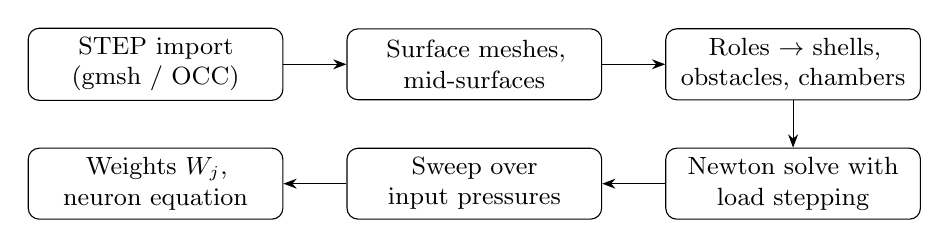
\begin{tikzpicture}[node distance=6mm and 8mm, >={Stealth},
  box/.style={draw, rounded corners, align=center, font=\small, minimum height=9mm, text width=30mm}]
\node[box] (cad) {STEP import\\(gmsh / OCC)};
\node[box, right=of cad] (mesh) {Surface meshes,\\mid-surfaces};
\node[box, right=of mesh] (build) {Roles $\to$ shells,\\obstacles, chambers};
\node[box, below=of build] (solve) {Newton solve with\\load stepping};
\node[box, left=of solve] (sweep) {Sweep over\\input pressures};
\node[box, left=of sweep] (fit) {Weights $W_j$,\\neuron equation};
\draw[->] (cad) -- (mesh); \draw[->] (mesh) -- (build); \draw[->] (build) -- (solve);
\draw[->] (solve) -- (sweep); \draw[->] (sweep) -- (fit);
\end{tikzpicture}
\caption{Pipeline of the simulator (Sections~\ref{sec:cad}, \ref{sec:energy}--\ref{sec:loadstep}
and \ref{sec:characterise}).}
\label{fig:pipeline}
\end{figure}

\paragraph{Units and conventions.} The application works in millimetres, newtons and
megapascals (so energies are in N\,mm), and it reports pressures in kPa. All pressures are
\emph{gauge} pressures: the surroundings are at $0$. A membrane face that touches no chamber
therefore sees zero pressure. The solver core (\code{membrane\_sim}) itself has no units; it
works in whatever consistent system the caller uses.

\paragraph{Code map.} Table~\ref{tab:code} links the sections of this document to the source
files.

\begin{table}[h]
\centering\small
\begin{tabular}{@{}lll@{}}
\toprule
File & Contents & Section \\
\midrule
\code{membrane\_sim/shell.py} & membrane and bending elements & \ref{sec:membrane}, \ref{sec:bending} \\
\code{membrane\_sim/fluid.py} & chamber volumes and pressure laws & \ref{sec:fluid} \\
\code{membrane\_sim/contact.py} & rigid obstacles, signed distance & \ref{sec:rigid} \\
\code{membrane\_sim/shell\_contact.py} & contact between membranes & \ref{sec:sheet} \\
\code{membrane\_sim/solver.py} & assembly and Newton iteration & \ref{sec:assembly}, \ref{sec:newton} \\
\code{membrane\_sim/environment.py} & load stepping & \ref{sec:loadstep} \\
\code{membrane\_sim/characterise.py} & weights and neuron equation & \ref{sec:characterise} \\
\code{app/cad.py}, \code{app/builder.py} & CAD import, meshing, coupling & \ref{sec:cad} \\
\code{app/sweep.py} & parameter sweeps & \ref{sec:sweep} \\
\bottomrule
\end{tabular}
\caption{Where each part of the formulation lives in the code.}
\label{tab:code}
\end{table}

%=====================================================================
\section{Equilibrium as energy minimisation}\label{sec:energy}
%=====================================================================

Let $\uu \in \mathbb{R}^{n}$ collect all unknowns: the current position $\x_a \in \mathbb{R}^3$ of
every mesh node $a$ of every shell and, for shells with bending, one rotation $\psi_e$ per mesh
edge (Section~\ref{sec:bending}). The rest positions are $\X_a$. Nodes on a clamped boundary are
fixed at their rest positions and removed from the unknowns.

Every force in the model is conservative, so the static equilibrium is a stationary point of the
total potential energy
\begin{equation}\label{eq:potential}
\Pi(\uu;\lambda) = \sum_{\text{shells}} \Big( U_{\text{mem}}(\uu) + U_{\text{bend}}(\uu) \Big)
  + E_{\text{rigid}}(\uu) + E_{\text{sheet}}(\uu)
  - \sum_{\text{chambers } v} \Phi_v\big(\dV_v(\uu);\lambda\big),
\end{equation}
where $U_{\text{mem}}$ and $U_{\text{bend}}$ are the strain energies of the shells,
$E_{\text{rigid}}$ and $E_{\text{sheet}}$ are penalty energies for contact with rigid bodies and
between membranes, $\dV_v$ is the volume change of chamber $v$, $\Phi_v$ is the work done by its
fluid, and $\lambda\in[0,1]$ is the load factor used to ramp the pressures. The solver finds a
point where
\begin{equation}
\R(\uu) = \frac{\partial \Pi}{\partial \uu} = \vect{0},
\end{equation}
using the tangent $\K = \partial^2\Pi/\partial\uu^2$, and it uses $\Pi$ itself as the merit
function of its line search (Section~\ref{sec:newton}). Stable equilibria are local minima of
$\Pi$. Because the formulation is variational, $\K$ is symmetric.

%=====================================================================
\section{Membrane energy}\label{sec:membrane}
%=====================================================================

Each shell is a mesh of three-node triangles with constant strain (CST). For a triangle with
rest vertices $\X_0,\X_1,\X_2$, an orthonormal in-plane basis is built from its rest normal
$\vect{N}_0$:
\begin{equation}
\vect{e}_1 = \frac{\X_1-\X_0}{\|\X_1-\X_0\|}, \qquad \vect{e}_2 = \vect{N}_0\times\vect{e}_1,
\qquad
\mathbf{D}_m = \begin{bmatrix} \vect{e}_1\cdot(\X_1-\X_0) & \vect{e}_1\cdot(\X_2-\X_0)\\
                               \vect{e}_2\cdot(\X_1-\X_0) & \vect{e}_2\cdot(\X_2-\X_0)\end{bmatrix}.
\end{equation}
With the current edge matrix $\mathbf{D}_s = [\x_1-\x_0,\; \x_2-\x_0] \in\mathbb{R}^{3\times2}$, the
surface deformation gradient and the right Cauchy--Green tensor are
\begin{equation}
\mathbf{F} = \mathbf{D}_s\mathbf{D}_m^{-1}\in\mathbb{R}^{3\times 2},\qquad
\mathbf{C} = \mathbf{F}^{\mathsf T}\mathbf{F}\in\mathbb{R}^{2\times2}.
\end{equation}
This is exact for arbitrarily large displacements and rotations \cite{bonet2008}. With $A_0$ the
rest area and $t$ the thickness, two materials are available.

\paragraph{Incompressible neo-Hookean (default, rubber).} For an incompressible sheet in plane
stress, the through-thickness stretch is $\lambda_3 = 1/J$ with $J^2 = \det\mathbf{C}$ (the area
stretch). Substituting it into the three-dimensional invariant
$I_1 = \tr\mathbf{C} + \lambda_3^2$ gives the energy per element
\begin{equation}\label{eq:neohookean}
U_{\text{mem}}^{e} = A_0\,\frac{\mu t}{2}\left(\tr\mathbf{C} + \frac{1}{\det\mathbf{C}} - 3\right)
+ T\,A,
\qquad \mu = \frac{E}{3},
\end{equation}
where $\mu=E/3$ is the shear modulus of an incompressible material ($\nu = 1/2$). The thickness
change is eliminated analytically, so no extra unknown is needed.

\paragraph{St.\ Venant--Kirchhoff.} On the Green--Lagrange strain
$\mathbf{E} = \tfrac12(\mathbf{C}-\I)$, with the plane-stress Lamé constant,
\begin{equation}
U_{\text{mem}}^{e} = A_0\,t\left(\frac{\bar\lambda}{2}(\tr\mathbf{E})^2 + \mu\,\mathbf{E}:\mathbf{E}\right)
+ T\,A,
\qquad \mu = \frac{E}{2(1+\nu)},\quad \bar\lambda = \frac{E\nu}{1-\nu^2}.
\end{equation}
This model is only meaningful for small strains. It is kept for comparison with linear plate
theory.

\paragraph{Pre-tension.} In both cases $T\,A$ adds an optional isotropic in-plane pre-tension $T$
(force per length) times the \emph{current} element area
$A = \tfrac12\|(\x_1-\x_0)\times(\x_2-\x_0)\|$. It acts like a surface tension. It is zero by
default.

\begin{remark}
A membrane without pre-tension or bending stiffness has no transverse stiffness in its flat
state: the tangent is singular at the start of every solve. The load stepping and the damped
Newton steps of Section~\ref{sec:newton} deal with this. It is also the physical reason why the
weights of Section~\ref{sec:characterise} behave singularly near zero pressure difference: a
clamped circular membrane under pressure $p$ (Hencky's problem \cite{hencky1915}) deflects as
$w \propto p^{1/3}$, so its displaced volume per unit pressure behaves like $p^{-2/3}$.
\end{remark}

%=====================================================================
\section{Bending energy}\label{sec:bending}
%=====================================================================

The \textbf{Shell} role adds bending stiffness through a geometrically nonlinear version of
Morley's constant-moment triangle \cite{morley1971}, written with mid-edge normals as in discrete
shell models \cite{grinspun2003,grinspun2006}. Every mesh edge $e$ carries one extra unknown, the
rotation $\psi_e$ of its mid-edge normal. The first attempt used an ``average face normal'' hinge
without $\psi_e$. That model's bending response depended on the orientation of the mesh, and the
$\psi_e$ unknowns remove that dependence. A test checks this
(\code{test\_bending\_energy\_is\_independent\_of\_mesh\_orientation}).

\paragraph{Edge rotations.} For triangle $f$ with current normal $\n_1$ and edge $k$ (opposite
vertex $k$, running from vertex $i$ to vertex $j$ with unit direction $\hat{\vect{e}}$), the
signed angle between $\n_1$ and a second normal $\n_2$ about the edge is
\begin{equation}
\theta_k = \operatorname{atan2}\big((\n_1\times\n_2)\cdot\hat{\vect{e}},\; \n_1\cdot\n_2\big).
\end{equation}
The rotation $\phi_k$ of the mid-edge normal relative to face $f$ depends on the edge type:
\begin{equation}
\phi_k = \begin{cases}
\tfrac12\theta_k + s_k\,\psi_e, & \text{interior edge, } \n_2 = \text{normal of the neighbouring face},\\[2pt]
\theta_k, & \text{clamped boundary edge, } \n_2 = \vect{N}_0 \text{ (rest normal)},\\[2pt]
\psi_e, & \text{free (hinged) boundary edge}.
\end{cases}
\end{equation}
Here $s_k=\pm1$ records the direction in which face $f$ traverses the edge, so the two faces that
share an interior edge see the same mid-edge normal. Here $\theta_k$ is the full dihedral angle,
so $\tfrac12\theta_k$ puts the mid-edge normal halfway between the two faces, and $\psi_e$ lets it
rotate further. A clamped edge is one whose two end nodes are both fixed while the shell's
boundary rotation is set to ``clamped''. Its mid-edge normal is held at the rest normal, and its
$\psi_e$ is removed from the unknowns.

\paragraph{Curvature and energy.} The face has the constant curvature tensor
\begin{equation}
\boldsymbol{\kappa} = \frac{1}{A_0}\sum_{k=1}^{3} l_k\,\phi_k\;\vect{m}_k\otimes\vect{m}_k,
\end{equation}
with rest edge lengths $l_k$ and in-plane outward edge normals $\vect{m}_k$ taken from the rest
state. With the change of curvature $\Delta\boldsymbol\kappa$ measured from the rest state
($\Delta\phi_k = \phi_k - \phi_k^0$, so curved CAD geometry is stress-free), the energy of a
linear-elastic plate,
\begin{equation}
U_{\text{bend}}^{e} = A_0\,\frac{D}{2}\Big(\nu\,(\tr\Delta\boldsymbol\kappa)^2 + (1-\nu)\,\Delta\boldsymbol\kappa:\Delta\boldsymbol\kappa\Big),
\qquad D = \frac{E t^3}{12(1-\nu^2)},
\end{equation}
becomes a quadratic form in $\Delta\boldsymbol\phi$. With $\tr(\vect{m}_i\otimes\vect{m}_i) = 1$ and
$(\vect{m}_i\otimes\vect{m}_i):(\vect{m}_j\otimes\vect{m}_j) = (\vect{m}_i\cdot\vect{m}_j)^2$,
\begin{equation}\label{eq:bendmatrix}
U_{\text{bend}}^{e} = \Delta\boldsymbol\phi^{\mathsf T}\mathbf{M}\,\Delta\boldsymbol\phi,
\qquad
M_{ij} = \frac{D}{2A_0}\,l_i l_j\Big(\nu + (1-\nu)(\vect{m}_i\cdot\vect{m}_j)^2\Big).
\end{equation}
$\mathbf{M}$ depends only on the rest geometry and is precomputed. All the geometric nonlinearity
sits in $\phi_k(\uu)$. For the neo-Hookean material $\nu=\tfrac12$, so $D = Et^3/9$.

%=====================================================================
\section{Fluid chambers}\label{sec:fluid}
%=====================================================================

\subsection{Volume change from the membranes alone}

A chamber is bounded partly by rigid walls and partly by membranes. Only its \emph{change} in
volume matters, and it can be computed from the membranes alone. Every membrane is clamped along
its boundary, so the rest mesh and the deformed mesh of the same membrane together close a
(possibly self-intersecting) volume, and that volume is exactly the volume the membrane has swept.
Using signed cone volumes about any fixed point $\vect{o}$,
\begin{equation}
V_{\text{cone}}(\x) = \frac16\sum_{\text{faces}} (\x_0-\vect{o})\cdot\big((\x_1-\vect{o})\times(\x_2-\vect{o})\big),
\end{equation}
the volume change of chamber $v$ is
\begin{equation}\label{eq:dV}
\dV_v(\uu) = \sum_{\text{shells } s \text{ on } v} \sigma_{s,v}\,\big(V_{\text{cone}}(\x_s) - V_{\text{cone}}(\X_s)\big),
\end{equation}
where $\sigma_{s,v}=+1$ if the shell's normal points out of the chamber (the chamber lies behind
the shell and pushes it along its normal) and $-1$ otherwise. The result does not depend on
$\vect{o}$ or on the rigid walls, which is why chamber walls never need a mesh. The code uses the
centroid of the rest mesh for $\vect{o}$, which limits round-off.

$\dV_v$ is a cubic polynomial in the node coordinates. Its gradient is
$\g_v = \partial\dV_v/\partial\uu$, which per face is
$\tfrac16\big(\x_1\times\x_2,\;\x_2\times\x_0,\;\x_0\times\x_1\big)$ (relative to $\vect{o}$). Its
Hessian is constant per face.

\subsection{Pressure laws}

Each chamber has a pressure law $P_v(\dV)$ with rest pressure $P_0$:
\begin{align}
\text{constant (input, vent)}:&\quad P = P_0 \quad(\text{vent: } P_0=0),\\
\text{sealed liquid}:&\quad P = P_0 - K\,(\dV + V_{\text{ex}}),
   \quad K = \frac{100\,s}{V_{\text{liq}}},\quad V_{\text{ex}} = V_{\text{body}} - V_{\text{liq}},
   \label{eq:liquid}\\
\text{sealed ideal gas}:&\quad P = (P_{\text{atm}} + P_0)\,\frac{V_g}{V_g + \dV} - P_{\text{atm}}.
   \label{eq:gas}
\end{align}
For the liquid, the user gives a stiffness $s$ in pressure per percent of volume change and a
liquid volume $V_{\text{liq}}$, which defaults to the volume of the CAD body. If the chamber holds
less liquid than its body volume ($V_{\text{ex}}>0$), the liquid is in suction and pulls the
membranes in; if it holds more, it inflates them. Water corresponds to $s\approx 22\,000$~kPa/\%.
Above about $1000$~kPa/\% the results hardly change, but the Newton iteration gets slower.

For the gas, Boyle's law is applied to the gas share only:
$V_g = (1-f)\,(V_{\text{body}} + V_{\text{ghost}})$, where $f$ is the liquid fraction (at most
$99\,\%$) and $V_{\text{ghost}}$ is an optional extra gas volume outside the modelled chamber, such
as tubing. Any liquid in the chamber is incompressible, so every volume change goes into the gas.
A state with $V_g+\dV\le 0$ gets infinite energy and is rejected by the line search. A user
supplied, differentiable law $P(\dV; P_0)$ is also supported.

\subsection{Potential, load and tangent}

The fluid's work is $\Phi_v(\dV) = \int_0^{\dV} P_v(s)\,\mathrm{d}s$. In closed form,
\begin{equation}
\Phi^{\text{liq}} = P_0\,\dV - K\left(V_{\text{ex}}\,\dV + \tfrac12\dV^2\right),\qquad
\Phi^{\text{gas}} = (P_{\text{atm}}+P_0)\,V_g\ln\frac{V_g+\dV}{V_g} - P_{\text{atm}}\,\dV,
\end{equation}
and a custom law is integrated with 16-point Gauss--Legendre quadrature. Differentiating
$-\Phi_v(\dV_v(\uu))$ gives the pressure load and its tangent:
\begin{equation}\label{eq:pressuretangent}
\frac{\partial(-\Phi_v)}{\partial\uu} = -P_v\,\g_v,\qquad
\frac{\partial^2(-\Phi_v)}{\partial\uu^2} = -P_v\,\frac{\partial^2\dV_v}{\partial\uu^2} - P_v'\,\g_v\g_v^{\mathsf T}.
\end{equation}
The force $P_v\g_v$ is exactly the follower pressure load, which acts normal to the \emph{deformed}
surface. The first tangent term is the usual load-stiffness term, and it is symmetric because
the load has a potential. The second term couples every node of a chamber to every other node. It
is a dense rank-one matrix, and Section~\ref{sec:assembly} handles it without forming it. Since
$P_v'\le0$ for every sealed chamber, $c_v = -P_v' \ge 0$ is a volumetric stiffness.

\subsection{Load path}

A fresh solve ramps every chamber from zero pressure: the solver uses $\lambda P_v(\dV)$ (and
likewise for the slope and potential). A warm-started solve (Section~\ref{sec:sweep}) starts from
a converged state with rest pressure $P_0^{\text{old}}$ and blends to the new rest pressure,
\begin{equation}
P_v^{\lambda}(\dV) = (1-\lambda)\,P_v(\dV; P_0^{\text{old}}) + \lambda\,P_v(\dV; P_0).
\end{equation}

%=====================================================================
\section{Contact with rigid bodies}\label{sec:rigid}
%=====================================================================

\subsection{Exact signed distance}

A rigid body is a closed, outward-oriented triangle mesh. For a point $\vect{p}$, the closest point
$\vect{q}$ on each candidate triangle is found with the region tests of Ericson
\cite{ericson2004}, which also report whether $\vect{q}$ lies on a face, an edge or a vertex. The
sign of the distance comes from the \emph{angle-weighted pseudo-normal} $\vect{N}_q$ of that
feature \cite{baerentzen2005}: the face normal on a face, the normalised sum of the two adjacent
face normals on an edge, and the sum of the incident face normals weighted by their angles at a
vertex. For a closed mesh this sign is exact:
\begin{equation}
d(\vect{p}) = \operatorname{sign}\big((\vect{p}-\vect{q})\cdot\vect{N}_q\big)\,\|\vect{p}-\vect{q}\|,
\qquad \nabla d = \operatorname{sign}(\cdot)\,\frac{\vect{p}-\vect{q}}{\|\vect{p}-\vect{q}\|}.
\end{equation}
$d<0$ inside the solid. An \emph{inverted} obstacle (a container whose inside is the free space)
flips the sign, and several obstacles combine by taking the minimum. The Hessian of the distance
is needed for a consistent tangent:
\begin{equation}
\nabla^2 d = \operatorname{sign}(\cdot)\,\frac{1}{|d|}\begin{cases}
\mathbf{0}, & \vect{q} \text{ on a face},\\
\I - \hat{\vect{u}}\hat{\vect{u}}^{\mathsf T} - \hat{\vect{t}}\hat{\vect{t}}^{\mathsf T}, & \vect{q} \text{ on an edge with direction } \hat{\vect{t}},\\
\I - \hat{\vect{u}}\hat{\vect{u}}^{\mathsf T}, & \vect{q} \text{ at a vertex},
\end{cases}
\end{equation}
with $\hat{\vect{u}} = (\vect{p}-\vect{q})/\|\vect{p}-\vect{q}\|$. On a face the Hessian is zero
because the face is flat.

\paragraph{Broad phase.} A nearest-vertex distance gives an upper bound on the closest distance,
and triangles whose bounding box is farther than that bound are skipped. Between Newton
iterations the candidate triangles of each node are cached in Verlet lists \cite{verlet1967}. At
a rebuild, each node keeps every triangle within its current distance plus $2\delta_s$ (the skin
$\delta_s$ is the larger of the contact reach and $1\,\%$ of the model size), and the list is
rebuilt as soon as any node has moved more than $\delta_s$. Until then the true closest triangle
is guaranteed to be in the list, so the cached query gives \emph{exactly} the result of a full
search. A test checks this (\code{test\_cached\_contact\_queries\_match\_the\_full\_search}).

\subsection{Penalty energy}

Each free node $a$ of a shell keeps a clearance $r_a$ from the obstacles: half the shell thickness,
reduced to the rest distance where the CAD geometry already starts closer than that. The contact
energy is a one-sided quadratic penalty,
\begin{equation}
E_{\text{rigid}} = \sum_a \tfrac12\,k\,A_a\,\min(d(\x_a)-r_a,\,0)^2,
\end{equation}
with $A_a$ the lumped nodal area (one third of the adjacent rest triangle areas). Weighting by
area makes $k$ a pressure per unit penetration, independent of the mesh. For an active node with
gap $\gamma_a = d-r_a<0$, the force and tangent are
\begin{equation}
\frac{\partial E}{\partial\x_a} = kA_a\,\gamma_a\,\nabla d,\qquad
\frac{\partial^2E}{\partial\x_a^2} = kA_a\left(\nabla d\,\nabla d^{\mathsf T} + \gamma_a\,\nabla^2 d\right).
\end{equation}

\paragraph{Choice of $k$.} A penalty always allows some penetration. At a contact pressure $p$ the
penetration is about $p/k$. The application chooses
\begin{equation}
k = \frac{\max(p_{\text{ref}},\,1\ \text{kPa})}{0.05\,t_{\min}},
\end{equation}
where $p_{\text{ref}}$ is the highest chamber pressure in the solve or sweep and $t_{\min}$ is the
thinnest part, so the penetration stays around $5\,\%$ of the thinnest thickness.

\paragraph{Clamp walls.} A membrane in CAD is usually clamped between rigid frame parts, so the
free nodes next to its fixed boundary start right at a rigid wall. These nodes sit on the on/off
kink of the penalty, and they made the Newton iteration cycle. Free nodes that share a triangle
with a fixed node and start within $1.25\,r_a$ of an obstacle are therefore excluded from rigid
contact.

%=====================================================================
\section{Contact between membranes}\label{sec:sheet}
%=====================================================================

Membranes can also touch each other (not themselves). Each sheet is a mid-surface with thickness
$t$, so node $a$ of sheet $A$ touches sheet $B$ when it comes closer than
$h = \tfrac12 t_A + \tfrac12 t_B$ to $B$'s mid-surface. As for rigid contact, $h$ is reduced to the
rest distance where the sheets already start closer, for example where they meet at a frame. For
every node--triangle pair within range, with $d$ the distance from the node to the closest point
of that triangle and penetration $\pi = h-d$,
\begin{equation}
E_{\text{sheet}} = \sum_{\text{pairs}} k A_a\,\varphi(\pi),\qquad
\varphi(\pi) = \begin{cases}
0, & \pi\le 0,\\
\dfrac{\pi^3}{6\delta}, & 0<\pi<\delta,\\[6pt]
\dfrac{\pi^2}{2} - \dfrac{\delta\pi}{2} + \dfrac{\delta^2}{6}, & \pi\ge\delta,
\end{cases}
\qquad \delta = 0.25\,h.
\end{equation}
The function $\varphi$ is the ordinary quadratic penalty with its stiffness ramped up over the
first $\delta$ of penetration. $\varphi$, $\varphi'$ and $\varphi''$ are continuous at $\pi=0$ and
at $\pi=\delta$ (the three values at $\delta$ are $\delta^2/6$, $\delta/2$ and $1$ from either
side), so a pair coming into contact does not make the tangent jump. \emph{All} triangles within
range contribute, not only the closest. With the closest only, the force jumps from one
triangle's vertices to its neighbour's when a node slides across an edge, and Newton cycled. Both
directions ($A$'s nodes on $B$ and $B$'s nodes on $A$) are included. The gradient and Hessian of
each pair's energy with respect to its twelve coordinates are exact
(Section~\ref{sec:assembly}).

\paragraph{No tunnelling.} A penalty can be stepped over: one large step can carry a node straight
through the other sheet to where the penalty is zero again. As in the continuous collision
handling of Incremental Potential Contact \cite{li2020ipc}, every line-search step is therefore
bounded conservatively. A node at distance $d$ from a triangle can only reach it if the two
approach each other by $d$, and in a step $\alpha\,\Delta\uu$ they approach by at most
$\alpha\big(\|\Delta\x_a\| + \max_{b\in\text{tri}}\|\Delta\x_b\|\big)$. The step fraction is
limited to
\begin{equation}
\alpha \le \min_{\text{pairs}} \frac{0.9\,d}{\|\Delta\x_a\| + \max_b\|\Delta\x_b\|},
\end{equation}
so no pair closes more than $90\,\%$ of its current distance in one step. Pairs whose bounding-box
distance already satisfies the bound are skipped without computing the exact distance.

%=====================================================================
\section{Assembly and exact derivatives}\label{sec:assembly}
%=====================================================================

Every energy above is written as a function of one element's coordinates: a membrane triangle
(9 values), a bending stencil (the triangle, its three opposite nodes and three edge rotations:
21 values), a pressure face (9), or a sheet-contact pair (12). The gradient and Hessian of each
element energy are obtained by automatic differentiation with \code{torch.func} (\code{grad},
\code{hessian}, vectorised over the elements with \code{vmap}) \cite{paszke2019}. The residual and
tangent are therefore the \emph{exact} derivatives of the discrete energy, which gives quadratic
Newton convergence without hand-derived tangent matrices. A test compares them with finite
differences of $\Pi$ (\code{test\_residual\_is\_energy\_gradient\_and\_tangent\_is\_its\_jacobian}).
Everything is computed in double precision.

The element contributions are assembled into a sparse matrix, and the rows and columns of fixed
unknowns are dropped. The chamber terms $P_v'\g_v\g_v^{\mathsf T}$ of
\eqref{eq:pressuretangent} are kept apart. Writing $\mathbf{U} = [\g_1,\dots,\g_m]$ for the
volume gradients of the $m$ chambers with $P_v'\neq0$ and $\mathbf{C} = \diag(c_v)$, the tangent
is
\begin{equation}
\K_{\text{full}} = \mathbf{A} + \mathbf{U}\mathbf{C}\mathbf{U}^{\mathsf T},
\end{equation}
where $\mathbf{A}$ is sparse. Linear systems are solved with a sparse LU factorisation of
$\mathbf{A}$ (SuperLU through SciPy \cite{virtanen2020}) and the Sherman--Morrison--Woodbury
identity \cite{hager1989}:
\begin{equation}\label{eq:woodbury}
\K_{\text{full}}^{-1}\vect{b} = \vect{y} - \mathbf{Z}\left(\mathbf{C}^{-1} + \mathbf{U}^{\mathsf T}\mathbf{Z}\right)^{-1}\mathbf{U}^{\mathsf T}\vect{y},
\qquad \vect{y} = \mathbf{A}^{-1}\vect{b},\quad \mathbf{Z} = \mathbf{A}^{-1}\mathbf{U}.
\end{equation}
This needs only $m$ extra back-substitutions and one small $m\times m$ solve.

%=====================================================================
\section{Newton iteration}\label{sec:newton}
%=====================================================================

At a fixed load factor $\lambda$, the solver iterates from the current state until
\begin{equation}
\|\R\| \le \tau_a + \tau_r\,\max\big(\|\vect{f}_{\text{int}}\|,\ \|\vect{f}_{\text{pres}}\|,\ \|\vect{f}_{\text{cont}}\|\big),
\end{equation}
with defaults $\tau_r = 10^{-8}$ and $\tau_a = 10^{-12}$. The reference is the largest of the
internal, pressure and contact force norms (free unknowns only). An iteration also counts as
converged when the undamped Newton step is below $10^{-10}$ times the model size (round-off
floor). Contact energies are only $C^1$ where a closest point crosses a triangle edge, which puts
a floor under the attainable residual. So when the residual has not halved for three iterations
and is within $1000$ times the tolerance, the iteration also stops as converged.

Each iteration tries the following steps in order, until one decreases the energy:

\begin{enumerate}[leftmargin=*]
\item \textbf{Newton step with second-order correction.} Solve $\K_{\text{full}}\,\vect{s} = -\R$
with \eqref{eq:woodbury} and search along $\vect{s}$, correcting every trial point as described
below.
\item \textbf{Levenberg--Marquardt steps.} If the Newton step fails, for example because the
tangent is indefinite or singular (a slack membrane, or a limit point), damp it:
$(\mathbf{A} + \mu\,\bar{a}\,\I + \mathbf{U}\mathbf{C}\mathbf{U}^{\mathsf T})\,\vect{s} = -\R$, with
$\bar a$ the mean absolute diagonal of $\mathbf{A}$. After a failure $\mu \leftarrow
\max(10\mu, 10^{-6})$, for up to four attempts. When the first attempt of an iteration is
accepted with a full step ($\alpha=1$), $\mu$ is reduced tenfold, or set to zero below $10^{-9}$.
$\mu$ carries over between iterations and load steps, so the first attempt is the undamped Newton
step only once the damping has died out.
\item \textbf{Gradient step.} As a last resort, search along the Jacobi-preconditioned steepest
descent direction $\vect{s} = -\R \oslash \big(|\diag\mathbf{A}| + (\mathbf{U}\circ\mathbf{U})\,|\vect{c}| + 10^{-8}\bar a\big)$,
with up to 40 backtracking steps. This always decreases the energy for a small enough step. If
it also fails, the Newton solve reports failure.
\end{enumerate}

\subsection{Line search on the energy}

Every candidate step is first scaled so that no coordinate moves more than $10\,\%$ of the model
size, and it is limited by the no-tunnelling bound of Section~\ref{sec:sheet}. A step length
$\alpha$ is then accepted under the Armijo condition \cite{nocedal2006}
\begin{equation}
\Pi(\uu_0 + \alpha\vect{s}) \le \Pi(\uu_0) + 10^{-4}\,\alpha\,\R^{\mathsf T}\vect{s}.
\end{equation}
If the condition fails, the next $\alpha$ is the minimiser of the quadratic through $\Pi(\uu_0)$,
the slope $\R^{\mathsf T}\vect{s}$ and $\Pi(\uu_0+\alpha\vect{s})$, kept within
$[0.1\alpha, 0.5\alpha]$. It is $\alpha/10$ when the trial energy is infinite (a gas pocket
squeezed to zero). A step whose energy change is within round-off of zero is also accepted if it
reduces the residual. \textbf{The energy is the only merit function.} Mixing in a
residual-decrease criterion made the iteration cycle as contact nodes switched in and out of
contact.

\subsection{Second-order volume correction}

Stiff sealed chambers need special treatment. A chamber's volume is a nonlinear function of the
node positions, so along a straight Newton step the actual volume change differs from the
linearised one by $O(\alpha^2\|\vect{s}\|^2)$. A nearly incompressible chamber (large $c_v$) turns
this small volume error into a large energy $\tfrac12 c_v e_v^2$. The line search then rejects
good Newton steps and convergence slows to a crawl. This is the Maratos effect known from
constrained optimisation, and the standard remedy is a second-order correction
\cite{nocedal2006}. Each trial point $\uu_0 + \alpha\vect{s}$ is moved back onto the linearised
volumes. With the volume error
\begin{equation}
e_v = \dV_v(\uu_0+\alpha\vect{s}) - \big(\dV_v(\uu_0) + \alpha\,\g_v^{\mathsf T}\vect{s}\big),
\end{equation}
the correction is the smallest change, in the norm of $\mathbf{A}$, that removes it to first
order:
\begin{equation}
\min_{\boldsymbol\delta}\ \tfrac12\boldsymbol\delta^{\mathsf T}\mathbf{A}\boldsymbol\delta
\quad\text{s.t.}\quad \mathbf{U}^{\mathsf T}\boldsymbol\delta = -\vect{e}
\qquad\Longrightarrow\qquad
\boldsymbol\delta = -\mathbf{Z}\left(\mathbf{U}^{\mathsf T}\mathbf{Z}\right)^{-1}\vect{e},
\end{equation}
where $\mathbf{Z} = \mathbf{A}^{-1}\mathbf{U}$ is already available from \eqref{eq:woodbury}. With
the correction, stiff and soft chambers converge in a similar number of iterations.

%=====================================================================
\section{Load stepping}\label{sec:loadstep}
%=====================================================================

The pressures are applied in load steps $\lambda = 0 \to 1$, with initial increment $1/N$
($N=10$ by default). After each converged step the state is stored; the application can play
these states back. The increment
\begin{itemize}[noitemsep]
\item grows by a factor $1.5$ (up to $1/N$) when a step converged in at most four iterations;
\item is halved, and the step retried from the last converged state, when Newton fails;
\item is considered too small below $10^{-3}$, at which point the solve stops and reports the
      last converged load factor.
\end{itemize}
A snap-through, such as a membrane ballooning past its limit point, has no nearby equilibrium, so
cutting the increment does not help. The first time the increment falls below $0.25/N$, the
solver makes one long ``relaxation'' attempt at the target load with five times the usual
iteration limit. The energy-descent iteration of Section~\ref{sec:newton} can then carry the
structure to its new equilibrium.

%=====================================================================
\section{From CAD to model}\label{sec:cad}
%=====================================================================

\paragraph{Import.} The STEP file is read with gmsh's OpenCASCADE kernel \cite{geuzaine2009}, in
millimetres. Every solid is one body. Names come from the product labels, or, for multi-body parts
from Fusion~360 whose names gmsh does not read, from the \code{MANIFOLD\_SOLID\_BREP} records of the
file.

\paragraph{Meshing.} Every body's boundary is triangulated with gmsh (Frontal--Delaunay, size set at
the CAD points). For membranes and shells the element size is the shortest \emph{in-plane} side of
the bounding box divided by a number of elements per side (default 10). For solids it is the
shortest side divided by that number, but never finer than the diagonal divided by three times
that number, so that thin rigid parts do not produce huge meshes. Each closed surface mesh is then
oriented outward: the faces of each connected component are made consistent by walking across
shared edges, the component is flipped if its signed volume is negative, and a component nested
inside an odd number of others is flipped again, because it bounds a cavity. The nesting depth is
found with the generalised winding number (below).

\paragraph{Mid-surfaces.} A membrane or shell body is replaced by its mid-surface. The body's
largest CAD face is taken as the primary face. From each of its nodes a ray is cast inward along
the vertex normal (Möller--Trumbore \cite{moller1997}) to the opposite faces, which measures the
local thickness $d$. The thickness is the median of these distances. Local values outside
$[\,\text{median}/3,\ 3\,\text{median}\,]$, or rays that miss, are replaced by the median, and
every node is moved inward by $\tfrac12 d$. The mid-surface keeps the orientation of the primary
face.

\paragraph{Boundary conditions.} By default all boundary nodes of the mid-surface are fixed (with
clamped rotations for shells). Alternatively, only boundary nodes within $0.75\,t$ of a rigid body
are fixed, which models a membrane clamped by a frame on some edges and free elsewhere.

\paragraph{Chamber coupling.} The software must find out which chambers act on which side of which
membrane. From the centroid of every mid-surface triangle, a probe point is placed on each side at
distance $\tfrac12 t + \max(\tfrac14 t, 10^{-3})$ along the normal. A probe lies inside a chamber
when the generalised winding number of the chamber's mesh exceeds $\tfrac12$
\cite{jacobson2013}. The winding number is evaluated as a sum of triangle solid angles
\cite{vanoosterom1983}:
\begin{equation}
w(\vect{p}) = \frac{1}{4\pi}\sum_{\text{tri}} 2\operatorname{atan2}\Big(\vect{a}\cdot(\vect{b}\times\vect{c}),\;
abc + (\vect{a}\cdot\vect{b})c + (\vect{a}\cdot\vect{c})b + (\vect{b}\cdot\vect{c})a\Big),
\end{equation}
with $\vect{a},\vect{b},\vect{c}$ the triangle vertices relative to $\vect{p}$ and $a,b,c$ their
lengths. If at least $30\,\%$ of the probes on one side are inside, the chamber is coupled to that
side of the membrane with the corresponding $\sigma$ of \eqref{eq:dV}. A chamber detected on both
sides has no net effect and is ignored with a warning. A warning is also given when the coverage
is below $90\,\%$, because the pressure is then applied to the whole membrane.

\paragraph{Chamber parameters.} Constant-pressure chambers are the inputs. Sealed liquid chambers
use \eqref{eq:liquid}, with $V_{\text{body}}$ the CAD volume. Sealed gas chambers use
\eqref{eq:gas} with $P_{\text{atm}} = 101.325$~kPa. Vents are constant-pressure chambers at zero.

%=====================================================================
\section{Parameter sweeps}\label{sec:sweep}
%=====================================================================

A sweep solves the model on a grid of one or two input-chamber pressures. The first point is a
fresh solve. Every following point is warm-started from the previous solution, ramping only the
change in rest pressure, with two load steps. If that fails, the point is solved fresh. One
penalty stiffness, chosen for the highest pressure in the sweep, is used for all points, so that
neighbouring points are consistent. Warm starting is several times faster, because contact is
already established. A test checks that it reaches the same state as a fresh solve
(\code{test\_warm\_start\_reaches\_the\_same\_state\_as\_a\_fresh\_solve}).

%=====================================================================
\section{Back-inferring the neuron equation}\label{sec:characterise}
%=====================================================================

The thesis models the input stage of the neuron as a sealed activation chamber $a$ whose
equilibrium pressure is a weighted average of the pressures acting on it:
\begin{equation}\label{eq:neuron}
p_a = \frac{\sum_j W_j\,p_j + W_0\,p_0 + B}{\sum_j W_j + W_0},
\end{equation}
where $W_j$ is the mechanical weight (compliance) of input $j$, $W_0$ the compliance of the
activation fluid itself about its rest pressure $p_0$, and $B$ a bias volume that is zero unless a
path contains a chamber that is not neutral at rest (Section~\ref{sec:bias}). In general the weights
depend on the pressure differences, $W_j = W_j(p_j - p_a)$, so \eqref{eq:neuron} is implicit in
$p_a$. This section describes how the weights are measured from simulations and fitted.

\subsection{Input paths}

A weight belongs to an \emph{input path}, not to a single membrane. Everything between an input
chamber and the activation chamber is lumped together. This can be one membrane, or, for the
bulk-modulus weight mechanism, membrane -- sealed weight chamber -- membrane. Paths are found from
the model's topology. Starting from every shell on the activation chamber, the far side of the
shell is examined:
\begin{itemize}[noitemsep]
\item no chamber there: the path reaches the surroundings, an \emph{ambient} input at $0$;
\item a constant-pressure chamber: the path reaches that input;
\item another sealed chamber: the search continues through the other shells of that chamber.
\end{itemize}
Shells that reach the same input form one path. A shell that reaches several inputs gets a
combined label.

\subsection{Secant and tangent weights}

For path $j$ with shells $s$ on the activation chamber, the volume pushed into the activation
chamber and the secant weight are
\begin{equation}
\dV_j = -\sum_{s\in j}\sigma_{s,a}\big(V_{\text{cone}}(\x_s) - V_{\text{cone}}(\X_s)\big),
\qquad
W_j = \frac{\dV_j}{p_j - p_a},
\end{equation}
and the activation fluid's own term is
\begin{equation}
W_0 = -\frac{\dV_a}{p_a - p_0},\qquad p_0 = P_a(0),
\end{equation}
which is zero for a perfectly incompressible fluid. Since
$\dV_a = -\sum_j \dV_j$, these definitions satisfy
$\sum_j W_j(p_j-p_a) + W_0(p_0-p_a) = \sum_j\dV_j + \dV_a = 0$ \emph{identically}. So
\eqref{eq:neuron} rebuilt from a point's own weights reproduces the simulated $p_a$ exactly. The
``$p_a$ from weights'' column of the sweep table checks the bookkeeping (paths, signs, volumes),
not the model. The weight is undefined where $p_j = p_a$ ($0/0$), and such points are left out.
Only $W_j$ is identified: pressure--volume data cannot separate an effective area $A_j$ from a
stiffness $K_j$ in $W_j = A_j/K_j$.

The \emph{tangent} weight is the local compliance $\partial\dV_j/\partial p_j$ with $p_a$ held
fixed. A unit increase of input pressure $p_j$ adds the load $\g_j$ (the volume gradient of input
chamber $j$). With the activation chamber's rank-one term removed from the tangent (fixed $p_a$),
and every other sealed chamber following its own law,
\begin{equation}
W_j^{\tan} = -\g_a^{\mathsf T}\,\K_{\neg a}^{-1}\,\g_j,
\qquad \K_{\neg a} = \mathbf{A} + \sum_{v\neq a} c_v\,\g_v\g_v^{\mathsf T},
\end{equation}
which is evaluated with \eqref{eq:woodbury}. For $W_0$ the tangent is $-1/P_a'(\dV_a)$. A test
checks $W^{\tan}$ against finite differences (\code{test\_tangent\_weight\_matches\_finite\_difference}).

\subsection{Sensitivity of the activation pressure}

For fixed weights, differentiating \eqref{eq:neuron} with respect to one weight gives
\begin{equation}\label{eq:sensitivity}
S_k = \frac{\partial p_a}{\partial W_k} = \frac{p_k - p_a}{\sum_j W_j + W_0},
\end{equation}
where $p_k-p_a$ becomes $p_0 - p_a$ for $W_0$. Increasing $W_k$ pulls $p_a$ towards $p_k$, and
$S_k=0$ where $p_k=p_a$: there, a weight has no influence on the activation pressure, however
large or nonlinear it is. This is exactly where the secant weight of a slack membrane is singular,
$W\propto |\Delta p|^{-2/3}$. The sweep plots colour every sample of $W_k$ by $|S_k|$, and the fit
below uses it as its weighting.

\subsection{Piecewise polynomial weights}

Each weight is fitted as a polynomial in its own pressure difference, $\Delta p_j = p_j - p_a$ for
an input and $\Delta p_0 = p_a - p_0$ for the activation fluid. There is \emph{one polynomial for
$\Delta p>0$ and one for $\Delta p<0$}, because a membrane deflecting towards the activation
chamber and one deflecting away from it can meet different obstacles. Each side is a separate
\emph{piece} with its own degree. A weight sampled on one side only uses that side's polynomial for
both signs.

\paragraph{Sensitivity-weighted least squares.} For one piece with samples $(\Delta p_i, W_i)$
and sensitivities $S_i$ from \eqref{eq:sensitivity}, evaluated with the sample's own weights, the
polynomial of degree $n$ minimises
\begin{equation}
\sum_i \left(\frac{|S_i|}{\max_k |S_k|}\right)^2\Big(\hat W(\Delta p_i) - W_i\Big)^2,
\qquad \hat W(\Delta p) = \sum_{m=0}^{n} c_m\,\Delta p^m.
\end{equation}
By \eqref{eq:sensitivity}, $|S_i|\,|\hat W - W_i|$ is to first order the error in $p_a$ caused by
the error in the weight. So the fit minimises the linearised activation-pressure error, not the
error in $W$. Without the weighting, the few samples just off $\Delta p = 0$, where $W$ is huge,
dominated the fit and forced high degrees with enormous coefficients, even though they barely
affect $p_a$. For conditioning, the fit is done in $\Delta p/\max|\Delta p|$ and rescaled
afterwards. Samples with $|\Delta p| \le 10^{-6}\max|\Delta p|$ are left out, and the degree is
capped at the number of distinct points minus one, and at 10.

\paragraph{Where the weighted average breaks down.} Equation~\eqref{eq:sensitivity} requires
$\sum_j W_j + W_0$ to be clearly positive. A sample whose weight sum is below $10^{-3}$ of
$\sum_k|W_k|$ is given no sensitivity and is left out of the polynomial fits (it is still part of the
tolerance check). The typical cause is an unmodelled bias, which the next subsection removes.

\subsection{Bias of non-neutral paths}\label{sec:bias}

A closed chamber \emph{inside} a path that is not neutral at rest pushes volume into the activation
chamber even when every pressure is equal. Examples are a gas weight chamber filled above ambient,
or a liquid one filled with more or less liquid than its volume (a chamber is neutral when its
pressure law gives zero gauge pressure at its rest volume). Where all pressures around the activation
chamber are equal, $p_a$ then still differs from them, which no weighted average can reproduce. The
secant weights $W_j = \dV_j/\Delta p_j$ are forced to cancel: in one test design,
$-152.6 + 109.7 + 42.6 + 0.3 \approx 0$\,mm$^3$/kPa at equal input pressures, which made $S_k$
diverge. Such a \emph{biased} path is modelled as
\begin{equation}
\dV_j = b_j + W_j(\Delta p_j)\,\Delta p_j,
\end{equation}
which puts $B = \sum_j b_j$ in \eqref{eq:neuron}. $W_j = (\dV_j - b_j)/\Delta p_j$ is then fitted like
any other weight.

$b_j$ is \emph{measured}, not fitted. When fitted as a free constant together with the weights, it
trades off against the polynomials. The tolerance on $p_a$ cannot tell them apart, and the fitted $B$
varied from $0.6$ to $18$~mm$^3$ with the chosen degrees on the test design. Instead, before the
sweep, one extra solve is made at the \emph{neutral state}: every constant-pressure input at the
activation chamber's rest pressure $p_0$. There an unbiased path pushes nothing, so what a biased
path pushes is its bias. The small pressure difference that remains is corrected to first order:
$b_j = \dV_j - W_j^{\tan}\Delta p_j$. On the test design this gives $b = 5.88$~mm$^3$, and the
corrected weights along the sweep become positive and peak at $\Delta p = 0$, as for a slack
membrane (1.75 \dots 15.4 \dots 1.88~mm$^3$/kPa), instead of passing through $-152.6$. The solve is
skipped when no path is biased.

\paragraph{Solving the equation.} Given the fitted weights, $p_a$ for an input set is a root of
\begin{equation}
r(p_a) = \sum_k \hat W_k(\Delta p_k)\,(p_k - p_a) + B = 0.
\end{equation}
Without a bias, a weighted average must lie between the lowest and highest pressure involved, so $r$
is sampled at 121 points on $[\min_k p_k,\ \max_k p_k]$. A bias can move $p_a$ outside that range, so
the interval is then widened by about $B/\sum_k \hat W_k(0)$. Every sign change is refined with
Brent's method.

Polynomial weights can make \eqref{eq:neuron} \emph{multivalued}: several activation pressures
satisfy it for the same inputs. Picking the root closest to the simulated $p_a$ would hide this,
since the equation, used on its own, has nothing to pick with. The fit therefore scores every sample
by its \emph{worst} root, so an equation only meets the tolerance if every activation pressure it
allows does. On the test design, the first version of this search accepted an equation that was
within $0.29$~kPa at every sample by its nearest root, but $1.2$~kPa off by another root.

\paragraph{Choosing the degrees.} The user sets a tolerance on the \emph{output} of the equation:
the fit must reproduce the simulated activation pressure of every sample within, by default,
$1$~kPa. The degrees are then made as low as possible. All pieces start at degree 0 (constant
weights). Two search strategies are available:
\begin{itemize}
\item \textbf{Lowest total order} (default): try every combination of piece degrees with total
      order $0, 1, 2, \dots$ and stop at the first total order at which some combination meets the
      tolerance, taking the one with the smallest maximum error. This is guaranteed to give the
      lowest possible total order.
\item \textbf{Biggest own error first} (greedy): while the tolerance is not met, add one degree to
      the piece with the largest \emph{own} error. That is the worst $p_a$ error when only that
      piece uses its polynomial and every other weight takes its sampled value. This is faster, but
      it can end at a higher total order, because errors of different pieces can cancel.
\end{itemize}
No piece is raised past the first degree that fits its points exactly. If the tolerance cannot be
met, the best combination found is returned and marked as such. The search is also limited to 2000
degree combinations, since an unreachable tolerance would otherwise make the exhaustive search try
millions of them. When the budget runs out, the best combination found so far is returned, marked as
stopped. The result is written out as LaTeX: \eqref{eq:neuron} with each weight given as a two-case
polynomial in its pressure difference, and $B$ with its parts $b_j$.

\paragraph{Checking between the sweep points.} The tolerance is checked at the sweep points only.
The application therefore also plots the simulated activation pressure with the fitted equation over
it: a curve for a one-input sweep, and a wireframe over the simulated surface for a two-input sweep.
The equation is evaluated on a finer grid than the sweep, and any extra roots are shown. A
high-degree polynomial can pass through every sweep point and still oscillate between them. That is
visible there and is a reason to sweep more densely rather than to tighten the tolerance.

\begin{remark}
When the activation fluid is nearly incompressible ($W_0 \ll W_j$), \eqref{eq:neuron} depends only
on the \emph{ratios} of the input weights: scaling every $W_j$ by the same factor leaves $p_a$
unchanged. A tolerance on $p_a$ then cannot pin down the absolute size of the weights, and fitted
weights can be off from the sampled ones by a common factor while still meeting the tolerance. The
fitted equation is correct as a map from input pressures to $p_a$. Individual fitted $W_j$ should
only be compared with each other.
\end{remark}

%=====================================================================
\section{Verification}\label{sec:verification}
%=====================================================================

The repository contains an automated test suite (\code{python -m pytest tests}). Grouped by what
they establish, the tests check that:
\begin{itemize}
\item \textbf{the discrete system is consistent}: the residual is the gradient of the energy and
      the tangent is its Jacobian, by finite differences, with active contact, for gas chambers,
      and for sheet contact;
\item \textbf{the elements converge to known solutions}: clamped square and circular plates
      against Kirchhoff plate theory \cite{timoshenko1959}; an inflated circular membrane against
      Hencky's solution \cite{hencky1915}; bending energy independent of mesh orientation;
\item \textbf{the chambers behave as intended}: the volume change of an imposed paraboloid; a
      very stiff sealed chamber gives the same state as a constant-pressure chamber at the same
      final pressure; a custom pressure law matches the equivalent built-in law; Boyle's law on the
      gas share; a gas pocket cannot be squeezed to zero; an under-filled liquid chamber pulls the
      membrane to its liquid volume;
\item \textbf{contact is correct}: signed distances match a brute-force search on convex and
      non-convex shapes; cached queries match the full search; a membrane inflates against a flat
      obstacle; an inflating sheet lifts another without passing through it;
\item \textbf{the solver is reproducible}: a warm-started solve reaches the same state as a fresh
      one;
\item \textbf{the characterisation is correct}: weights of direct, ambient and bulk-modulus paths
      rebuild the activation pressure; a stiffer weight fluid transfers more; the tangent weight
      matches finite differences; the fitted equation uses the lowest degrees that meet the
      tolerance, with one polynomial per sign; a measured bias enters the equation exactly; a
      multivalued equation is judged by its worst root; the search stops at its budget and can be
      cancelled; cancelling weight sums give no sensitivity;
\item \textbf{the CAD pipeline works}: part names, closed outward meshes, mid-surfaces, measured
      thickness, chamber--membrane coupling and project save/load on a generated test assembly.
\end{itemize}

%=====================================================================
\section{Limitations}\label{sec:limitations}
%=====================================================================

\begin{itemize}
\item \textbf{Static only.} There is no inertia, damping or fluid flow, so the switching dynamics
      of the output stage and the flow through resistors are outside the model.
\item \textbf{Lumped chambers.} Every chamber has one uniform pressure. Where a chamber covers only
      part of a membrane, the pressure is still applied to the whole membrane (with a warning).
\item \textbf{Penalty contact.} Contact allows a small penetration (about $5\,\%$ of the thinnest
      thickness by default) and makes the tangent stiff. There is no friction and no
      self-contact of a sheet. Sheet contact can still stall under very large pushes (one test of
      this case does not yet pass).
\item \textbf{Nearly incompressible chambers} use a stiff linear pressure law rather than a mixed
      formulation with the pressure as an unknown. Very high stiffness is therefore
      ill-conditioned, although the second-order correction keeps it usable.
\item \textbf{Material models.} Only incompressible neo-Hookean and St.\ Venant--Kirchhoff sheets are
      available, with no viscoelasticity or damage, and there is no check that stretches stay
      within the material's limits.
\item \textbf{Robustness.} The globalised Newton method has no convergence guarantee. Snap-through
      and hard contact cases can still stall before full load; the solve then reports the last
      converged load factor rather than a result at full load.
\end{itemize}

%=====================================================================
\begin{thebibliography}{99}
%=====================================================================

\bibitem{baerentzen2005}
J.~A. B{\ae}rentzen and H.~Aan{\ae}s,
``Signed distance computation using the angle weighted pseudonormal,''
\emph{IEEE Transactions on Visualization and Computer Graphics}, vol.~11, no.~3, pp.~243--253, 2005.

\bibitem{bonet2008}
J.~Bonet and R.~D. Wood,
\emph{Nonlinear Continuum Mechanics for Finite Element Analysis}, 2nd~ed.
Cambridge University Press, 2008.

\bibitem{ericson2004}
C.~Ericson, \emph{Real-Time Collision Detection}. Morgan Kaufmann, 2004.

\bibitem{geuzaine2009}
C.~Geuzaine and J.-F. Remacle,
``Gmsh: a 3-D finite element mesh generator with built-in pre- and post-processing facilities,''
\emph{International Journal for Numerical Methods in Engineering}, vol.~79, no.~11, pp.~1309--1331, 2009.

\bibitem{grinspun2003}
E.~Grinspun, A.~N. Hirani, M.~Desbrun, and P.~Schr{\"o}der,
``Discrete shells,'' in \emph{Proc.\ ACM SIGGRAPH/Eurographics Symposium on Computer Animation}, 2003, pp.~62--67.

\bibitem{grinspun2006}
E.~Grinspun, Y.~Gingold, J.~Reisman, and D.~Zorin,
``Computing discrete shape operators on general meshes,''
\emph{Computer Graphics Forum}, vol.~25, no.~3, pp.~547--556, 2006.

\bibitem{hager1989}
W.~W. Hager, ``Updating the inverse of a matrix,''
\emph{SIAM Review}, vol.~31, no.~2, pp.~221--239, 1989.

\bibitem{hencky1915}
H.~Hencky, ``{\"U}ber den Spannungszustand in kreisrunden Platten mit verschwindender Biegungssteifigkeit,''
\emph{Zeitschrift f{\"u}r Mathematik und Physik}, vol.~63, pp.~311--317, 1915.

\bibitem{jacobson2013}
A.~Jacobson, L.~Kavan, and O.~Sorkine-Hornung,
``Robust inside-outside segmentation using generalized winding numbers,''
\emph{ACM Transactions on Graphics}, vol.~32, no.~4, 2013.

\bibitem{li2020ipc}
M.~Li, Z.~Ferguson, T.~Schneider, T.~Langlois, D.~Zorin, D.~Panozzo, C.~Jiang, and D.~M. Kaufman,
``Incremental potential contact: intersection- and inversion-free, large-deformation dynamics,''
\emph{ACM Transactions on Graphics}, vol.~39, no.~4, 2020.

\bibitem{moller1997}
T.~M{\"o}ller and B.~Trumbore, ``Fast, minimum storage ray-triangle intersection,''
\emph{Journal of Graphics Tools}, vol.~2, no.~1, pp.~21--28, 1997.

\bibitem{morley1971}
L.~S.~D. Morley, ``The constant-moment plate-bending element,''
\emph{Journal of Strain Analysis}, vol.~6, no.~1, pp.~20--24, 1971.

\bibitem{nocedal2006}
J.~Nocedal and S.~J. Wright, \emph{Numerical Optimization}, 2nd~ed. Springer, 2006.

\bibitem{paszke2019}
A.~Paszke \emph{et al.}, ``PyTorch: an imperative style, high-performance deep learning library,''
in \emph{Advances in Neural Information Processing Systems 32}, 2019.

\bibitem{timoshenko1959}
S.~Timoshenko and S.~Woinowsky-Krieger, \emph{Theory of Plates and Shells}, 2nd~ed. McGraw-Hill, 1959.

\bibitem{vanoosterom1983}
A.~van Oosterom and J.~Strackee, ``The solid angle of a plane triangle,''
\emph{IEEE Transactions on Biomedical Engineering}, vol.~BME-30, no.~2, pp.~125--126, 1983.

\bibitem{verlet1967}
L.~Verlet, ``Computer `experiments' on classical fluids. I. Thermodynamical properties of Lennard-Jones molecules,''
\emph{Physical Review}, vol.~159, no.~1, pp.~98--103, 1967.

\bibitem{virtanen2020}
P.~Virtanen \emph{et al.}, ``SciPy 1.0: fundamental algorithms for scientific computing in Python,''
\emph{Nature Methods}, vol.~17, pp.~261--272, 2020.

\end{thebibliography}

\end{document}
